% Copyleft 2010 by Walter Vargas <walter@covetel.com.ve>

\documentclass[9pt]{beamer}
\usepackage{listings}
\lstset{
    language=HTML 
}
\lstset{
    basicstyle=\scriptsize, 
    stringstyle=\ttfamily,
    showstringspaces=false, 
    numbers=left,
    numberstyle=\scriptsize,
    tabsize=2,
}

% Configuración de la apariencia. 

\usetheme{Szeged}
\usecolortheme{beaver}
\usefonttheme[onlylarge]{structurebold}
\setbeamerfont*{frametitle}{size=\normalsize,series=\bfseries}

\usepackage{color}
\definecolor{lightgray}{rgb}{.9, .9, .9}
\definecolor{darkgray}{rgb}{.4, .4, .4}
\definecolor{purple}{rgb}{0.65,  0.12,  0.82}
\definecolor{azulito}{HTML}{0066CC}

\lstdefinelanguage{HTML}{
keywords={xml, DOCTYPE, head,  body, html, return,  this}, 
keywordstyle=\color{azulito}\bfseries, 
ndkeywords={title, option, form, textarea, table, th, tr, td, p, br, input,
button, frame, iframe, div, optgroup, select, fieldset,  legend, h1, h2, h3,
h4, h5, h6, p, blockquote, address, em,strong, abbr, acronym, cite, dfn, code,
kbd, samp, var, q, ul, li, dl, dt, dd, strong, span, add, attr, is, prev,
parent, children, parents, gt, find, lt, eq, not,  contains, filter, visible,
hidden, nth, even, odd, css}, 
ndkeywordstyle=\color{blue}\bfseries, 
identifierstyle=\color{black}, 
sensitive=false, 
comment=[l]{//}, 
morecomment=[s]{/*}{*/}, 
stringstyle=\color{azulito}\ttfamily, 
morestring=[b]', 
morestring=[b]"
}

\lstset{
language=HTML, 
backgroundcolor=\color{lightgray}, 
extendedchars=true, 
basicstyle=\scriptsize\ttfamily, 
showstringspaces=false, 
showspaces=false, 
numbers=left, 
numbersstyle=\footnotesize, 
numbersep=9pt, 
tabsize=2, 
breaklines=true, 
showtabs=false, 
captionpos=b 
}


% Paquetes
\usepackage[utf8]{inputenc}
\usepackage[spanish]{babel}


% Titulo
\title[WebDesign] {Diseño Web | Tecnologías Involucradas}
\author[Walter Vargas]{ info@covetel.com.ve \inst{1}}
\subtitle{Capa de Presentación CSS}
\institute[covetel.com.ve]{ \inst{1} Cooperativa Venezolana de Tecnologías Libres R.S. }
\date

\begin{document}

\begin{frame} % (fold)
    \titlepage 
\end{frame}

\begin{frame} % (fold)
    \tableofcontents
\end{frame}

\section{Principios básicos de las hojas de estilo en cascada}

\subsection{Principios} % (fold)

% subsection Principios (end)

\begin{frame}{Las ventajas de CSS} % (fold)
    \begin{itemize}
        \item Mayor control de la tipografía  del diseño de la página. 
        \item Menos trabajo
        \item Documentos potencialmente más pequeños
        \item Documentos potencialmente más accesibles
        \item HTML de presentación ya esta en vía de desaparecer
        \item Tiene buen soporte
    \end{itemize}
\end{frame}

\begin{frame}{Como funciona CSS} % (fold)
    \begin{itemize}
        \item Se crea el documento XHTML o HTML 
        \item Se escriben las reglas de estilo para definir el aspecto 
        \item Se vinculan los estilos al documento. 
    \end{itemize}
\end{frame}


\begin{frame}[fragile]{Hojas de estilo incrustadas \texttt{<style> </style>}} % (fold)
    Un método más compacto para agregar hojas de estilo,  es incrustar un
    bloque de estilo en la parte superior del documento HTML. 

    \textbf{Atributos no comunes}
    \begin{itemize}
        \item \texttt{media='all|aural|braille|handheld|print|projection|screen|tty|tv'}
        \item \texttt{title='text'}
        \item \texttt{type='tipo de contenido'} (\textit{requerido})
    \end{itemize}

    \begin{lstlisting}
<html>
<head>
<style type="text/css">
h1 {color:red;}
p {color:blue;}
</style>
</head>
<body>
<h1>Header 1</h1>
<p>A paragraph.</p>
</body>
</html>
    \end{lstlisting}

\end{frame}


\begin{frame}[fragile]{Hojas de estilo externas} % (fold)
    El método mas eficiente de utilizar CSS es reunir todas las reglas de
    estilo en un documento de texto independiente y crear vínculos a ese
    documento desde todas las páginas de un sitio. \\[0.5cm]

    Este modo permite hacer cambios de estilo homogéneos en todo el sitio
    editando un solo documento. \\[0.5cm]

    El documento de hoja de estilo es un documento de texto con al menos una
    regla de estilo. \\[0.5cm]

    El documento de hoja de estilo puede contener comentarios, como por
    ejemplo: 

    \begin{lstlisting}
/* Esto es un comentario */
    \end{lstlisting}
\end{frame}

\begin{frame}[fragile]{Utilizar un Link} % (fold)
    El método con mejor soporte para hacer referencia a hojas de estilo es
    crear un vínculo al documento CSS utilizando el elemento \texttt{link} en
    la cabecera \texttt{head} del documento. 

\begin{lstlisting}
<head>
    <link rel="stylesheet" type="text/css" href="theme.css" />
</head>
\end{lstlisting}
    
    El atributo \texttt{rel} define la relación del documento externo con el
    documento actual, el atributo \texttt{href} indica la URL del documento de
    hoja de estilo. Los autores pueden vincular más de una hoja de estilo al
    documento. 
\end{frame}

\begin{frame}[fragile]{Importar} % (fold)
    Una alternativa a los vínculos es importar una hoja de estilo externa a un
    documento utilizando la función \texttt{@import} en el elemento
    \texttt{style}

    \begin{lstlisting}
<style type="text/css"> 
    <!-- 
    @import url(http://www.example.com/stylesheet.css);
    -->
</style> 
    \end{lstlisting}
\end{frame}


\subsection{Conceptos fundamentales} % (fold)

\begin{frame}{Conceptos fundamentales} % (fold)
    Para familiarizarse con el comportamiento de CSS es importante comprender
    sus conceptos claves.

    \begin{itemize}
        \item Estructura y herencia documentales 
        \item Reglas de estilo en conflicto: la "cascada"
        \item Tipos de elementos
        \item El modelo de cajas. 
    \end{itemize}
\end{frame}

\begin{frame}{Estructura y herencia documentales}
    Los documentos XML, XHTML y HTML tienen una jerarquía implícita. Por
    ejemplo, el documento raíz \texttt{html} suele contener un \texttt{head} y
    un \texttt{body} y el \texttt{body} a su vez contiene distintos elementos a
    nivel de bloque como párrafos \texttt{p}. Esta jerarquía puede visualizarse
    como un árbol, separándose en ramas desde la raíz. La siguiente figura
    muestra la estructura de un documento XHTML muy sencillo.

\end{frame}

\begin{frame}{Estructura y herencia documentales} % (fold)
    \begin{center}
    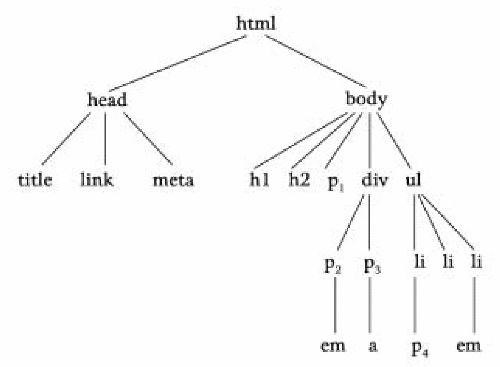
\includegraphics[scale=0.5]{imgs/htmlestructura.png}
    \end{center}
\end{frame}

\begin{frame}{La relación padre-hijo} % (fold)
    La estructura del documento se convierte en un árbol genealógico cuando se
    hace referencia a las relaciones entre elementos. Un elemento que esta
    contemplado directamente por otro elemento es el \textbf{hijo} de éste. En
    la figura anterior el elemento \texttt{p1} es hijo de \texttt{body} y
    \texttt{body} es su \textbf{padre}. Los elementos que tienen el mismo
    padre, son \textbf{hermanos}. En el ejemplo el elemento \texttt{li} es el
    hijo de \texttt{ul} y el resto de los elementos \texttt{li} son sus
    hermanos. \\[0.5cm]

    La relación \textbf{padre-hijo} es fundamental para el funcionamiento de
    CSS
\end{frame}


\begin{frame}{Herencia} % (fold)
    En la relación con las relaciones estructurales está el concepto de
    herencia, por la cual la mayoría de los estilos pasan de un elemento a sus
    descendientes. Esto indica en otras palabras que un hijo puede heredar
    propiedades de su padre. \\[0.5cm]

    Por ejemplo, si una regla de estilo aplica un color para un elemento
    \texttt{ul}, también aplica para para todos sus hijos \texttt{li}. \\[0.5cm]

    En CSS la mayoría de las propiedades se heredan, pero algunas como
    márgenes y fondos no. 
\end{frame}


\begin{frame}{Reglas de estilo en conflicto: la cascada} % (fold)
    Es posible y común que los elementos de un documento tengan instrucciones
    de presentación de distintas fuentes. Es posible entonces, que surjan
    conflictos. El grupo de trabajo que desarrolló CSS ya anticipó esta
    situación y concibió un sistema jerárquico que asigna distintos pesos a
    distintas fuentes de información de estilo. \\[0.1cm]

    La \textbf{cascada} de hojas de estilo en cascada se refiere a lo que
    ocurre si varias fuentes de información de estilo concurren por el control
    de los elementos de una página; la información de estilo se transmite hasta
    que es ignorada por un comando de estilo con más peso. \\[0.1cm]

    La cascada ordena proporcionar un conjunto de reglas para resolver
    conflictos entre hojas de estilo concurrentes. Cuando un agente de usuario
    encuentra un elemento mira a todas las declaraciones de estilo que pueda
    tener aplicadas y las ordena de acuerdo al origen de la hoja de estilo, a
    la especificidad de los selectores y al orden de la regla para determinar
    cuál aplicar. 
\end{frame}


\begin{frame}{Origen de la hoja de estilo} % (fold)
    Los navegadores dan distinto peso a las hojas de estilo de estas fuentes,
    listadas de menor a mayor peso: 

    \begin{itemize}
        \item Hojas de estilo del agente de usuario
        \item Hojas de estilo del lector
        \item Hojas de estilo del autor
        \item Declaraciones de estilo \texttt{!important} del lector.
    \end{itemize}
\end{frame}


\begin{frame}[allowframebreaks, fragile]{Jerarquía de pesos adicionales } % (fold)

    Tras considerar la fuente de la hoja de estilo hay otra jerarquía de pesos
    que se aplica a las hojas de estilo creadas por el autor del
    documento. \\[0.1cm]

    Los puntos de origen en las hojas de estilo del autor tienen también
    distintos pesos (recuerde que todos los estilos del autor ignoran los
    estilos del agente de usuario y del lector a no ser que el lector marque el
    estilo como \texttt{!important})\\[0.1cm]

    Esta lista señala el peso de las distintas declaraciones de estilo del
    autor, de menor a mayor peso. En otras palabras, las reglas de estilo que
    están al final de la lista ignoran a las primeras. 
    
    \begin{enumerate}
        \item \textbf{Hojas de estilo externas vinculadas (utilizando el atributo
        \texttt{link})}: Si hay varias hojas de estilo vinculadas, las reglas
        de estilo de las hojas de estilo listadas por debajo en el documento
        tendrán preferencia sobre las listadas por encima. Por ejemplo, si un
        documento HTML vincula a dos hojas de estilo,  de este modo: 
        \begin{lstlisting}
<head>
<link rel="stylesheet" href="style1.css" type="text/css" />
<link rel="stylesheet" href="style2.css" type="text/css" /> 
</head>
        \end{lstlisting}
        Si una regla de estilo indicada en \texttt{style2.css} esta en
        conflicto con una regla de estilo de \texttt{style1.css}, la regla de
        \texttt{style2.css} tendrá preferencia porque la hoja de estilo está
        listada por debajo en el documento fuente. 

        \item  \textbf{Hojas de estilo externas importadas (utilizando
        \texttt{@import})}: La información de estilo importada ignora los
        estilos vinculados en el header. Si hay varias directivas \texttt{@import} las
        reglas indicadas en las hojas de estilo que estén por debajo en la
        lista ignoran las que están por encima. 

        \item \textbf{Hojas de estilo incrustadas (con el elemento
        \texttt{<style>})}:
        Los estilos aplicados a un documento determinado ignoran las
        reglas establecidas externamente. 

        \item \textbf{Estilos en línea (utilizando el atributo \texttt{style=}
        en una etiqueta de elemento)}: Los estilos en línea ignoran todas las
        demás declaraciones de estilo que puedan hacer referencia a ese
        elemento, con una excepción: 

        \item \textbf{Declaraciones de estilo marcadas como
        \texttt{!important}}: Cualquier estilo marcado como \texttt{!important}
        ignora todas las reglas de estilo en conflicto. Lo único que puede
        ignorar una regla importante de una hoja de estilo de autor es una
        regla importante creada por el usuario. 
    \end{enumerate}
        
        Ejemplo utilizando la directiva \texttt{!important}: 

        \begin{lstlisting}
p {color: blue !important; }
        \end{lstlisting}

        En la siguiente gráfica podemos ver el orden de prioridades. \\[0.5cm]

        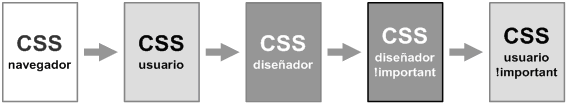
\includegraphics[scale=0.55]{imgs/css-orden.png}
\end{frame}

\begin{frame}[allowframebreaks, fragile]{Especificidad del selector} % (fold)
    La cascada continua a nivel de reglas, en el siguiente ejemplo, hay dos
    reglas que hacen referencia al elemento \texttt{strong} \\[0.5cm]
\begin{lstlisting}
strong {color: red;}
h1 strong {color: blue;}
\end{lstlisting}

    El agente de usuario asigna distintos tipos de niveles de peso a los
    distintos tipos de selectores. Cuanto más específico sea el selector más
    peso se le dará para ignorar las las declaraciones en conflicto. Para el
    ejemplo anterior todo el texto \texttt{strong} del documento se renderizará
    en rojo. Sin embargo, si el texto \texttt{strong} aparece dentro de una
    cabecera \texttt{h1} se renderizará en azul porque un elemento de un
    contexto determinado es más específico y tiene más peso. 

    Esta es una lista de tipos de selector en orden de peso de menor a mayor.

    \begin{enumerate}
        \item Selectores de elementos y pseudoelementos específicos (por
        ejemplo \texttt{p} o \texttt{first-letter}) 
        \item Selectores contextuales (p.e. \texttt{h1 strong})
        \item Selectores de clase (p.e. \texttt{p.special})
        \item Selectores ID (p.e. \texttt{p\#intro})
    \end{enumerate}

    Recuerde que todas las reglas marcadas como \texttt{!important} ignorarán
    reglas en conflicto sea cual sea su especifidad u orden. 
\end{frame}

\begin{frame}[allowframebreaks, fragile]{Orden de las reglas} % (fold)
    Por último, cuando los estilos se han ordenado por autor,  método de
    vinculación y especificidad, puede seguir habiendo conflictos dentro de una
    única fuente de hoja de estilo. Cuando una hoja de estilo contiene varias
    reglas en conflicto de igual peso, la que esté de última en lugar tiene más
    peso e ignora al resto. Por ejemplo, en el siguiente ejemplo, todas las
    cabeceras de primer nivel del documento serían rojas porque se impone la
    última regla. 

\begin{lstlisting}
h1 {color: green;}
h1 {color: blue;}
h1 {color: red;}
\end{lstlisting}
    
    Ya se habló de este principio de \textbf{el último gana} en relación a
    varios elementos \texttt{link} y comandos \texttt{@import}. También se
    aplica en un solo bloque de declaración. Por ejemplo. 

\begin{lstlisting}
div#side {border-color: gray; 
    border-color-top: black; }
\end{lstlisting}

\end{frame}

\begin{frame}[allowframebreaks]{Elementos de bloque y en línea} % (fold)
    En XHTML, la distinción entre los elementos a nivel de bloque y en línea se
    basa en reglas de contención o, en otras palabras, en función del
    anidamiento de elementos en otros documentos. En general, los elementos a
    nivel de bloque pueden contener elementos elementos en línea y elementos de
    bloque, mientras que los elementos en linea solo pueden contener texto y
    otros elementos en linea. \\[0.2cm]

    Sin embargo, algunos de estos elementos de bloque deben cumplir reglas
    especiales en XHTML, como son los párrafos, las cabeceras, y direcciones
    (\texttt{address}) solo pueden contener elementos en línea y contenido.\\[0.5cm]

    En CSS, sin embargo, la noción de \textbf{nivel de bloque} y \textbf{en
    linea}  es puramente de presentación visual. \texttt{block} e
    \texttt{inline} son dos posibles roles de maestra en pantalla utilizados
    para indicar a los agentes de usuario cómo presentar el documento en el
    diseño. \\[0.5cm]

    Un elemento a nivel de bloque de CSS (\texttt{display: block}) siempre
    genera saltos antes y después de él. Llena el ancho disponible del elemento
    padre que lo contiene sea el ancho del cuerpo del documento o un espacio
    menor definido como el de un \texttt{div}. No puede emplazar nada junto a
    un elemento de bloque en el flujo normal del documento. \\[0.5cm]

    Los elementos en línea CSS (\texttt{display: inline}) no generan saltos de
    linea. Aparecen en el flujo de la linea y sólo pasarán a otra línea si no
    tienen espacio. \\[0.5cm]

    A diferencia de las nociones de XHTML de bloque y en linea, un elemento a
    nivel de bloque CSS puede estar anidado en un elemento en línea y
    viceversa. Al utilizar CSS cualquier elemento XHTML (o XML) puede
    convertirse a nivel de bloque o en línea. 

\end{frame}

\begin{frame}[allowframebreaks, lstlisting]{Introducción al modelo de cajas} % (fold)
    El modelo de cajas constituye la piedra angular del sistema de formateo
    visual de CSS. Es un concepto fundamental para comprender el funcionamiento
    de las hojas de estilo.  \\[0.5cm]

    De acuerdo al modelo de cajas todos los elementos, a nivel de bloque o en
    línea, generan una caja rectangular alrededor llamada \textbf{caja de
    elemento} (aunque las cajas de bloque y de línea se tratan ligeramente de
    manera distinta). \\[0.5cm]

    Pueden aplicarse propiedades como bordes, márgenes y fondos (entre otras) a
    la caja de un elemento. Las cajas también pueden utilizarse para posicionar
    elementos y diseñar la página.\\[0.5cm]

    Las cajas de elementos están hechas de cuatro componentes principales. En
    el núcleo de la caja está el contenido del elemento. El contenido está
    rodeado por cierta cantidad de relleno, sigue el borde rodeado por el
    margen como puede verse en las figuras \ref{fig:box1} y \ref{fig:box2}.

    \begin{figure}
        \caption{Modelo de Cajas}
        \label{fig:box1}
        \centering
        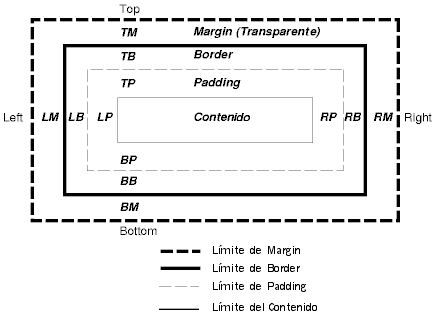
\includegraphics[scale=0.55]{imgs/boxmodel1.png}\footnote{Esta imágen se
        utiliza con autorización de \url{http://www.sidar.org/recur/desdi/traduc/es/css/box.html}}
    \end{figure}
    
    \begin{figure}[H]
        \caption{Modelo de Cajas 3D}
        \label{fig:box2}
        \centering
        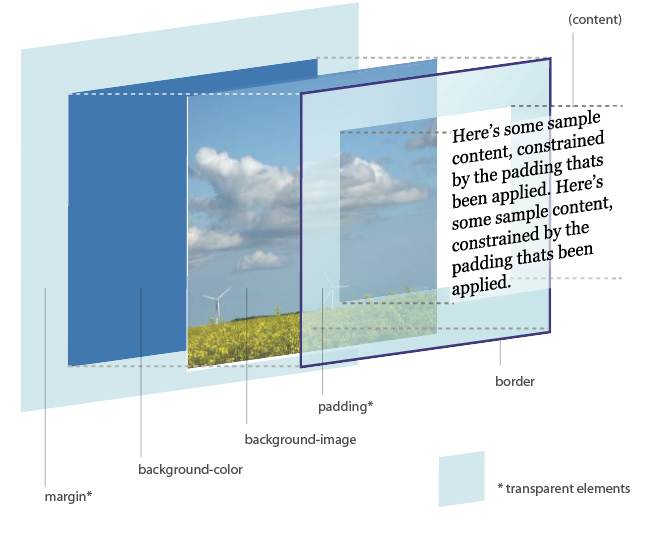
\includegraphics[scale=0.3]{imgs/boxmodel2.png}\footnote{Esta imágen se
        utiliza con autorización de \url{http://www.hicksdesign.co.uk/boxmodel/}}
    \end{figure}

    \textbf{ Característias fundamentales del modelo de caja que merece la pena
    destacar: }\\[0.5cm]

    \begin{enumerate}
        \item Relleno, bordes y márgenes son opcionales. Si ajusta a cero sus
        valores se eliminan de la caja. 
        \item El área de relleno es el espacio entre el borde del área de
        contenido y el borde (si lo hay). Cualquier color o imagen de fondo
        aplicados al elemento se extenderá por toda el área de relleno. 
        \item Los bordes se generan con propiedades de estilo, que especifican
        su estilo, ancho y color. Cuando un borde tiene huecos, el color o
        imagen de fondo aparece a través de esos huecos. En otras palabras, los
        fondos se extienden tras el borde hasta el borde exterior. 
        \item Los margenes siempre son transparentes, lo que significa que el
        color de fondo o el patrón del elemento padre se mostrará a través de
        ellos. El límite del margen (el borde exterior del elemento) no es
        visible,  pero es una cantidad calculada. 
        \item El ancho de un documento solo se aplica al ancho del área de
        contenido. Esto significa que si especifica que un elemento debería
        tener una anchura de 200px, los contenidos reales se mostrarían con una
        anchura de 200px, y los anchos acumulativos del relleno, el borde y los
        márgenes, se sumarían a esa cantidad.
        \item Se puede cambiar el estilo de los lados superior, derecho,
        inferior, e izquierdo de una caja de elemento por separado. Por
        ejemplo, puede añadir un borde a la parte inferior de un elemento o
        solo a los lados derecho e izquierdo. 
    \end{enumerate}

    
\end{frame}




\end{document}
